\documentclass{article}
\usepackage{main,times}

\usepackage{amsmath}
\usepackage{amssymb}
\usepackage{graphicx}
\usepackage{booktabs}
\usepackage{array}
\usepackage{url}
\usepackage{subcaption}
\usepackage{float}
\usepackage[colorlinks=true,
            linkcolor=blue,
            citecolor=blue,
            urlcolor=blue]{hyperref}

\title{
\makebox[\linewidth][c]{%
    \raisebox{-0.22\height}{%
        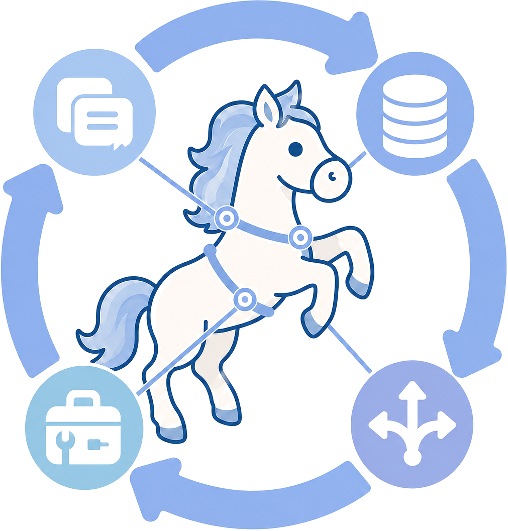
\includegraphics[height=1.2em]{Figures/logo.pdf}%
    }%
    \hspace{0.3em}%
    Harness Continual Learning: Continual%
}\\[0.10em]
\makebox[\textwidth][c]{%
    \hspace{-2.50em}%
    Adaptation Beyond Model Parameters%
}
}

\author{
Borui Kang$^{1}$,
Jinrui Gu$^{1}$,
Junhan Lv$^{1}$,
Wenbin Li$^{1}$\thanks{Corresponding author},
Lei Wang$^{2}$,
Yang Gao$^{1}$
\\[0.5em]
$^{1}$State Key Laboratory for Novel Software Technology,
Nanjing University, China
\\
$^{2}$University of Wollongong, Australia
\qquad
\\
}

\iclrfinalcopy

\begin{document}

\maketitle


\begin{abstract}
Continual learning has largely been model-centric, treating model parameters as
the state that changes with sequential experience. Modern agents can also adapt
through a harness of prompts, memories, tools, skills, and routing rules.
Because these contents jointly shape later execution, a harness update can
disrupt previously reliable behavior even when the model is frozen. This raises
a new question: how can an agent continually improve its state outside the model
while retaining behavior acquired earlier? We formulate \emph{Harness
Continual Learning} (HCL), a new continual learning paradigm in which the
harness evolves around a frozen foundation model, and define the resulting loss
of earlier behavior as \emph{harness-level forgetting}. We instantiate HCL with four execution-facing components: the Task Interface, Experience Memory, Capability Map, and Adaptive Router. We further introduce \emph{guarded harness evolution} to separate update generation from state commitment. A Continual Optimizer proposes candidate harnesses from post-execution feedback, and a Continual Evaluator commits the resulting candidate harness only after checking current improvement, historical retention, and validity. Experiments on textual reasoning, multimodal perception, and open-world interaction demonstrate capability accumulation and
failure recovery, with relative gains exceeding 10\% over corresponding
baselines in multiple settings. Component ablations assess the contribution of
each harness component, while controlled retention sweeps reveal measurable
harness-level forgetting and show that the stability--plasticity trade-off can
be explicitly adjusted.
\end{abstract}

\section{Introduction}
\label{sec:introduction}

Continual learning studies how a system acquires capabilities from sequential
experience while retaining previously learned behavior
\citep{delange2021continual,wang2024comprehensive,
shi2024continuallearninglargelanguage}. Existing formulations realize this
process mainly by changing model parameters, representations, or architectural
components. 
We refer to this established view as \emph{model-centric continual learning}.


The rise of agentic AI introduces another source of adaptation: an external \emph{harness} that determines how a foundation model receives information, retrieves experience, and acts
\citep{jimenez2024swebenchlanguagemodelsresolve,
xie2024osworldbenchmarkingmultimodalagents,
xu2025theagentcompanybenchmarkingllmagents,
chen2026standalonellmsintegratedintelligence,
li2026agentharness,
meng_agent_2026_harness}. 
Prompts, memories, tool and skill specifications, and routing policies can persist and evolve across interactions even
when the foundation model remains frozen. Agent adaptation is therefore no
longer confined to model state: harness state can also accumulate
experience and reshape future behavior. \emph{This makes the harness a new
object of continual learning research, extending the study of continual
adaptation beyond model parameters}, as illustrated in
Figure~\ref{fig:hcl_concept}.

\begin{figure*}[t]
\centering
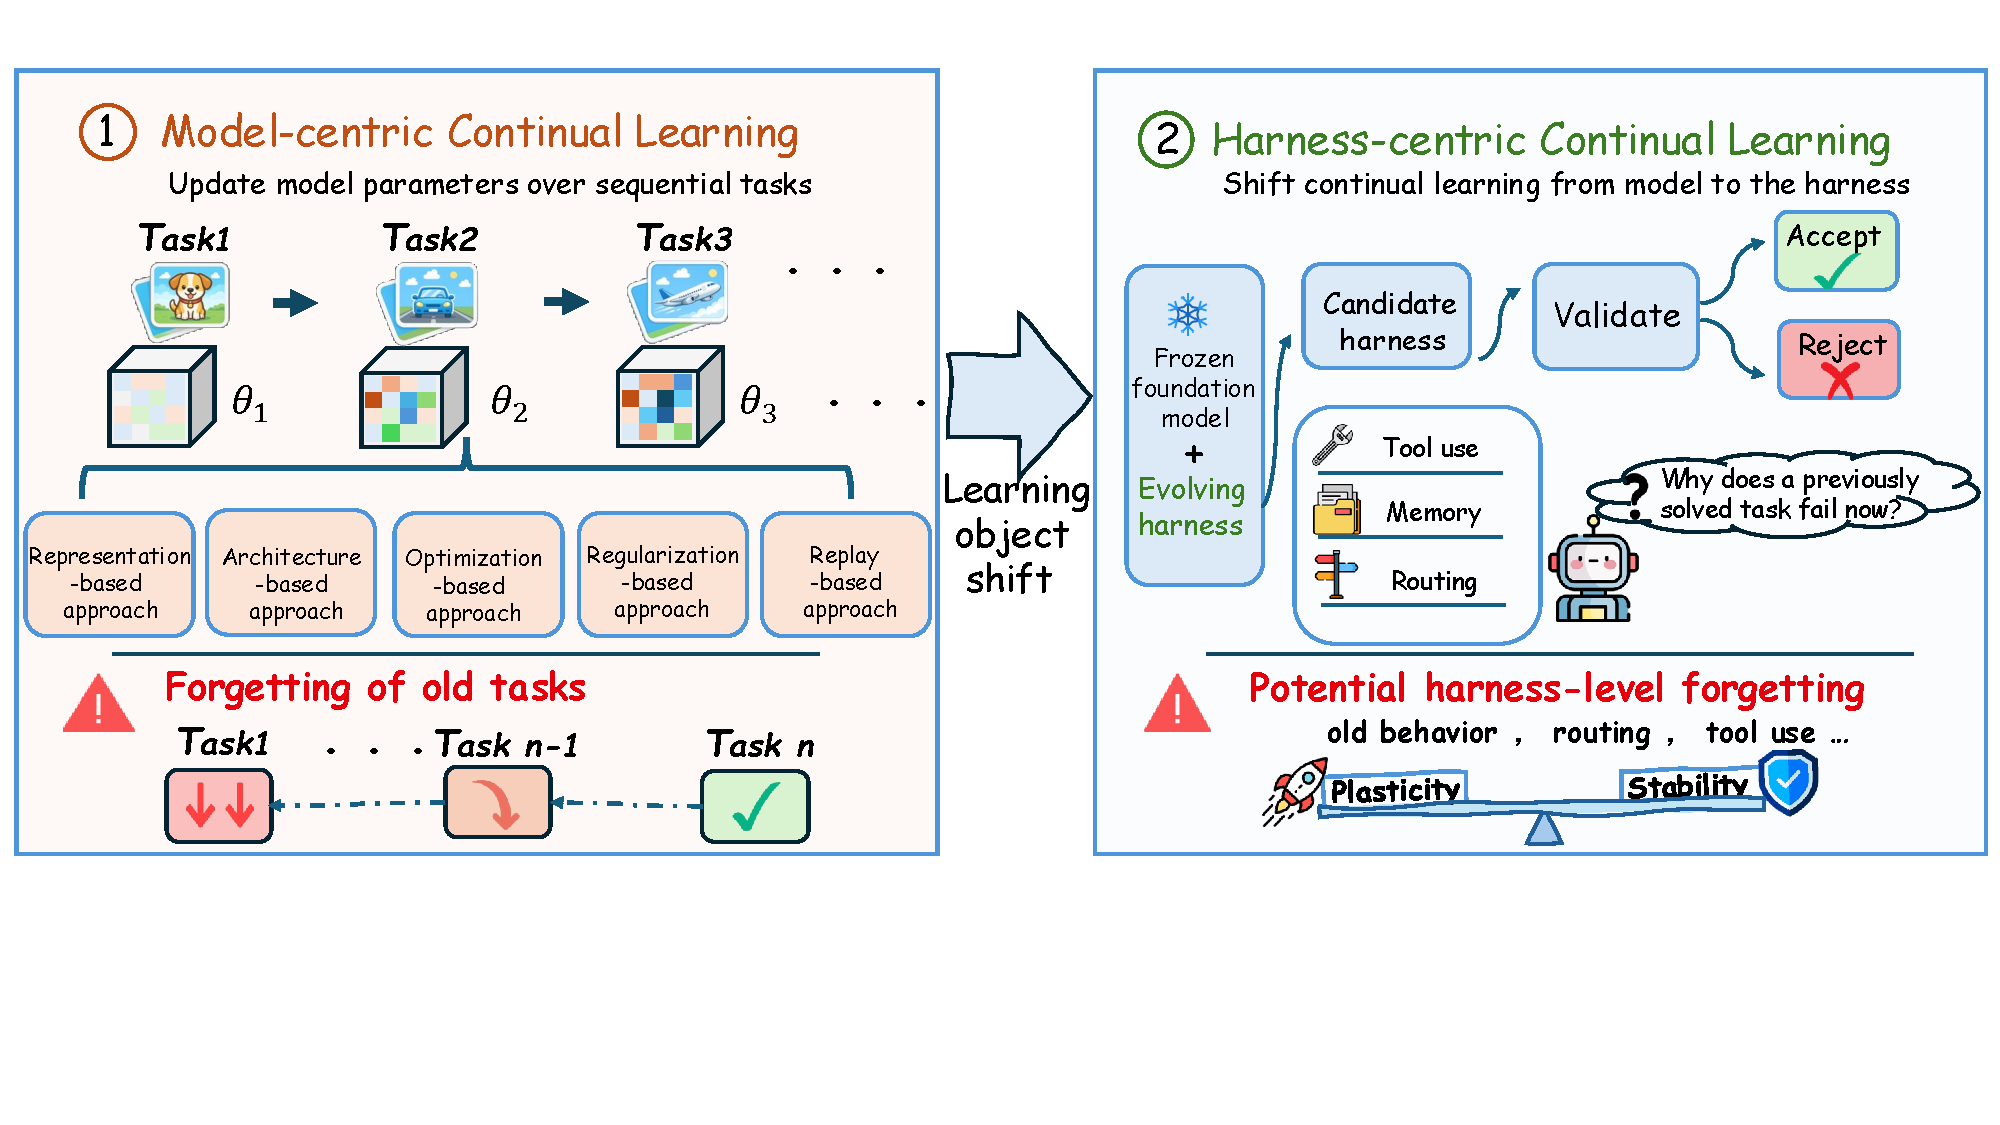
\includegraphics[width=\linewidth]{Figures/intro.pdf}
\caption{
The shift in the object of continual learning. Model-centric methods update
model parameters $\theta$ over sequential experience. HCL instead updates harness
state around a frozen foundation model. In both settings, adaptation can
improve new behavior while interfering with behavior acquired earlier.
}
\label{fig:hcl_concept}
\end{figure*}

We formalize this new direction as \emph{Harness Continual Learning} (HCL), a
continual learning paradigm that acquires and retains capabilities by
sequentially updating harness state around a frozen foundation model.
Conventional harness optimization typically searches for prompts, functions,
or workflows that improve a current objective
\citep{zhang2024agentoptimizer,zhang2025aflowautomatingagenticworkflow}. HCL instead studies a sequence of updates. Its concern is not only whether the next update helps the current
interaction, but also whether the evolving harness retains behavior that
earlier updates made reliable.
This setting introduces a distinct retention problem. Harness components are
coupled in execution: a memory update can change the evidence retrieved for an earlier query; a skill revision can alter tool use; and a routing edit can break a previously successful workflow. An update that helps recent cases can therefore turn an earlier correct answer, valid tool call, or successful action trajectory into a failure without changing the foundation model. We call this phenomenon \emph{harness-level forgetting}. It extends the classical stability--plasticity problem from model state to harness state.

To study continual adaptation under this retention requirement, we develop an
HCL framework with two parts. First, we define the Task Interface, Experience
Memory, Capability Map, and Adaptive Router as the harness state and learning
object of HCL. These components are jointly versioned and determine how the
agent processes information, reuses experience and capabilities, and organizes
execution. Second, \textit{guarded harness evolution} governs state transitions through two modules: a Continual Optimizer that proposes candidate harnesses from post-execution feedback, and a Continual Evaluator that determines whether those candidates can be committed. The two parts jointly operationalize HCL: the former defines what is learned, while the latter controls how the harness is updated over time. Only a candidate harness that improves current validation performance while satisfying the historical-retention budget and validity constraints is committed as the deployed state. This proposal--evaluation--commitment process makes retention an explicit condition of harness adaptation, mitigating harness-level forgetting while controlling
the stability--plasticity trade-off.

We evaluate HCL across textual reasoning, multimodal perception, and open-world interaction. The
results show that harness evolution can accumulate capabilities and support failure recovery, while
also producing measurable harness-level forgetting. Historical-retention budgets shift the operating
point between adaptation and retention, and more permissive updates do not necessarily produce a
stronger final harness. In this work, our contributions are as follows:
\begin{itemize}

\item We propose and formalize \emph{Harness Continual Learning} as a new
continual learning paradigm, shifting the learning object from model state to harness state around a frozen foundation model.

\item We identify \emph{harness-level forgetting} and develop \emph{guarded harness evolution}, in which a Continual Optimizer proposes candidate harnesses and a
Continual Evaluator controls commitment through current, historical, and
validity checks.

\item We show across textual reasoning, multimodal perception, and open-world
interaction that harness evolution supports capability accumulation and
failure recovery while exhibiting measurable forgetting and a controllable
stability--plasticity trade-off.

\end{itemize}
\section{Related Work}
\label{sec:related_work}

\subsection{Harness Engineering}
\label{sec:harness_structure}

Contemporary agent systems place a runtime harness around a foundation model
to turn inference into task-directed execution
\citep{li2026agentharness,meng_agent_2026_harness,
he_harness_2026,zhou2026harness}. Across implementations, persistent runtime
contents commonly serve four functions. An \emph{interface} converts raw
instructions, observations, documents, or multimodal inputs into a form the
agent can use. \emph{Memory} stores interaction records, summaries, and
reusable guidance. A \emph{capability registry} describes tools, APIs,
environment actions, and learned skills together with their invocation
conditions. A \emph{router or workflow controller} selects relevant memories
and capabilities, orders their use, and assembles the execution context.
Environment adapters execute actions, and task-specific validators check
outcomes at the boundary of the pipeline
\citep{gu2026modelscalingscalingscaling,
chen2026harnessxcomposableadaptiveevolvable}.


Existing systems develop different parts of this structure. ReAct couples
reasoning with environment interaction
\citep{yao2023react}. Toolformer, MRKL, and HuggingGPT expose and coordinate
external capabilities
\citep{schick2023toolformerlanguagemodelsteach,
karpas2022mrklsystemsmodularneurosymbolic,
shen2023hugginggptsolvingaitasks}. MemGPT, Reflexion, and Voyager retain
experience as memory, feedback, or executable skills
\citep{packer2024memgptllmsoperatingsystems,shinn2023reflexion,voyager}.
Together, these components form a coupled execution pipeline. The interface
shapes what the router sees. Memory and capability descriptions determine what
it can select. The resulting workflow determines how the model acts.

Harness engineering also uses execution feedback to revise prompts,
declarative programs, memories, tool-use policies, skills, and workflows
\citep{zhou2023largelanguagemodelshumanlevel,
khattab2023dspycompilingdeclarativelanguage,
abuzakuk2026optimizingagenticworkflowsusing,
schick2023toolformerlanguagemodelsteach,shinn2023reflexion,voyager,
zhong2026skilllearnbenchbenchmarkingcontinuallearning,
zhang2026skillflowbenchmarkinglifelongskilldiscovery}. Recent work broadens this process to
configuration search, cross-layer failure diagnosis, and sustained agent
improvement
\citep{zhang2026selfharnessharnessesimprove,
chen2026failedtrajectoriesreliablellm,
yao2026harnessbenchmeasuringharnesseffects,
liu2026adaptiveautoharnesssustainedselfimprovement}. These systems show that a
harness is editable and can improve with experience. Their main objective,
however, is usually the quality of a component or the next configuration on a
current task or target distribution. Repeated improvement alone does not
provide a general retention criterion for the full harness state
\citep{lin2026harnessupdatingharnessbenefit}. Our work differs by treating the
entire mutable harness as a unified continual learning state and by making
retention across committed updates an explicit objective.

\subsection{Model-Centric Continual Learning}

Model-centric continual learning adapts a model to a non-stationary stream of
tasks or data while seeking to retain capabilities acquired from earlier
experience. Its central challenge is catastrophic forgetting, which arises
when learning new knowledge disrupts knowledge encoded by the model
\citep{kirkpatrick2017overcoming,delange2021continual,
wang2024comprehensive,kangdon}. Representation-based approaches learn features or
prompts that remain useful across tasks
\citep{wang2022l2p,wang2022dualpromptcomplementarypromptingrehearsalfree}.
Recent analysis also examines how these internal representations shift across a
learning sequence \citep{kim2025measuringrepresentational}.
Architecture-based approaches isolate, expand, or select model components to
reduce interference between tasks
\citep{liu2026cp,lu2024revisitingarchitectures}.
Optimization-based approaches alter the update trajectory or constrain
gradients using information from earlier tasks
\citep{lopezpaz2017gem,abbes2026replaygradient,
shang2025divideorthogonalize}.
Regularization-based approaches penalize changes to parameters or functions
that support old behavior
\citep{kirkpatrick2017overcoming,lewandowski2025spectralregularization}.
Replay-based approaches retain or reconstruct earlier examples and mix them
with new data
\citep{urettini2025ocar,wang2025cutreplay,
yue2025tdgr,bellitto2024saliencyreplay}. Recent
work extends these families
to large language models and broader knowledge streams, but the state being
learned remains model knowledge, representations, architectures, or parameters
\citep{liang2026gated,zhang2026multi}. Our work
moves the continual learning object outside the model. The foundation model
parameters remain frozen, while the harness state evolves under explicit
acquisition and retention constraints.

\section{Harness Continual Learning}
\label{sec:hcl_framework}


\begin{table}[t]
\centering
\footnotesize
\caption{
Execution functions and updatable contents of the four jointly versioned
components in the deployed harness $H_n$.
}
\label{tab:hcl_state_overview}

\setlength{\tabcolsep}{3pt}
\renewcommand{\arraystretch}{0.98}

\begin{tabular}{
    >{\raggedright\arraybackslash}p{0.18\textwidth}
    >{\raggedright\arraybackslash}p{0.33\textwidth}
    >{\raggedright\arraybackslash}p{0.39\textwidth}
}
\toprule
Component
& Function during execution
& Contents updated in HCL \\
\midrule

Task Interface $I_n$
& Transforms raw interactions into structured representations.
& Prompts, task templates, and parsing and normalization rules. \\

\addlinespace[3pt]

Experience Memory $M_n$
& Provides concrete interactions and abstract guidance for reuse.
& Raw interaction records and LLM-generated Abstract Memory entries. \\

\addlinespace[3pt]

Capability Map $C_n$
& Provides external operations and reusable inner skills.
& Inner skills extracted from Abstract Memory. \\

\addlinespace[3pt]

Adaptive Router $R_n$
& Selects and organizes memory and capabilities.
& Routing prompts, selection criteria, and workflow templates. \\

\bottomrule
\end{tabular}
\end{table}

\subsection{Definition and Problem Setting}
\label{sec:problem_setting}


Consider a fixed foundation model $F_{\theta}$ and a harness $H_n$ deployed at
interaction step $n$. The model parameters $\theta$ remain unchanged, whereas
a committed harness update affects subsequent interactions. We define
\emph{Harness Continual Learning} as the problem of sequentially updating
the deployed harness to acquire new behavior while retaining behavior that was
reliable before the update. Previously reliable behavior may be a correct
response, a valid tool call, or an action trajectory that satisfies an
environment goal. Retention requires such behavior to remain successful after
later harness updates when evaluated under the same input and execution
conditions.
This setting differs from conventional harness engineering, which typically
optimizes a prompt, tool configuration, or workflow for a current objective.
HCL instead studies a sequence of deployed harnesses. 

At interaction step $n$, $\mathbf{u}_n$ denotes the raw interaction, such as an
instruction, an observation, or a multimodal input. The harness transforms
$\mathbf{u}_n$ into the structured interaction $\mathbf{i}_n$. Guided by the
frozen foundation model, it then combines $\mathbf{i}_n$ with selected memory
and capabilities to assemble the execution context $\mathbf{z}_n$. The model
and external runtime execute $\mathbf{z}_n$ to produce the outcome
$\mathbf{y}_n$. Post-execution feedback is denoted by $\mathbf{f}_n$. We
collect these interaction-level objects as
\begin{equation}
\label{eq:interaction_evidence}
\mathbf{e}_n
=
\left(
\mathbf{u}_n,
\mathbf{i}_n,
\mathbf{z}_n,
\mathbf{y}_n,
\mathbf{f}_n
\right).
\end{equation}
The Optimizer provides the foundation model $F_{\theta}$ with an update rule, the deployed harness, and the available interaction evidence as context for generating a candidate harness::
\begin{equation}
\label{eq:hcl_candidate_transition}
\widetilde{H}_{n+1}
=
\mathcal{O}_{F_{\theta}}
\left(
H_n,
\mathbf{e}_n
\right).
\end{equation}
The candidate remains separate from the deployed harness until a commitment
decision is made. Let $G_n \in \{0,1\}$ denote this decision. The deployed
harness evolves as
\begin{equation}
\label{eq:hcl_general_transition}
H_{n+1}
=
\begin{cases}
\widetilde{H}_{n+1}, & G_n = 1,\\
H_n, & G_n = 0.
\end{cases}
\end{equation}
Therefore, a candidate affects later interactions only when it is committed.
Our framework realizes HCL in two parts. First, it defines the deployed harness state $H_n$ by specifying its mutable contents and versioning them jointly. Second, it controls the update from $H_n$ to ${H}_{n+1}$ by checking current improvement,
historical retention, and validity before commitment.


\subsection{Harness State for Continual Learning}
\label{sec:evolving_state}

The design of the HCL state builds on established mechanisms from prior
harness and agent systems, including prompt-based task interfaces, persistent
memory, tool and skill registries, and routing or workflow controllers
\citep{li2026agentharness,he_harness_2026}. Rather than inheriting the architecture of any single system, HCL organizes
these recurring execution functions into four jointly versioned components, whose mutable contents evolve from sequential experience under explicit acquisition and retention constraints.

Accordingly, HCL organizes the mutable harness state as
\begin{equation}
\label{eq:hcl_state}
H_n
=
\left(
I_n,
M_n,
C_n,
R_n
\right),
\end{equation}
where $I_n$, $M_n$, $C_n$, and $R_n$ denote the Task Interface, Experience
Memory, Capability Map, and Adaptive Router, respectively. At interaction step
$n$, $H_n$ represents the complete harness currently deployed. Its prompts and
processing rules, stored experience, reusable skills, and routing
specifications persist across interactions and jointly determine how the agent
handles future tasks.

Although these four execution functions are common in agent harnesses, HCL
differs in how their mutable contents are learned and deployed. Because a
change to one component may interact with the others and affect both new and
previously learned behavior, HCL treats all proposed changes as one complete
candidate harness. The candidate replaces $H_n$ only after it satisfies current improvement, historical retention, and validity requirements. Otherwise, none of its changes enters the deployed harness. HCL therefore turns harness contents into a coordinated mechanism for continual learning rather than a collection of independently edited artifacts.

Table~\ref{tab:hcl_state_overview} summarizes the execution function of each
component and the contents that can be updated through continual interaction.
Figure~\ref{fig:hcl_framework} shows how these components support execution and
how post-execution feedback initiates a candidate harness. 


\begin{figure*}[t]
\centering
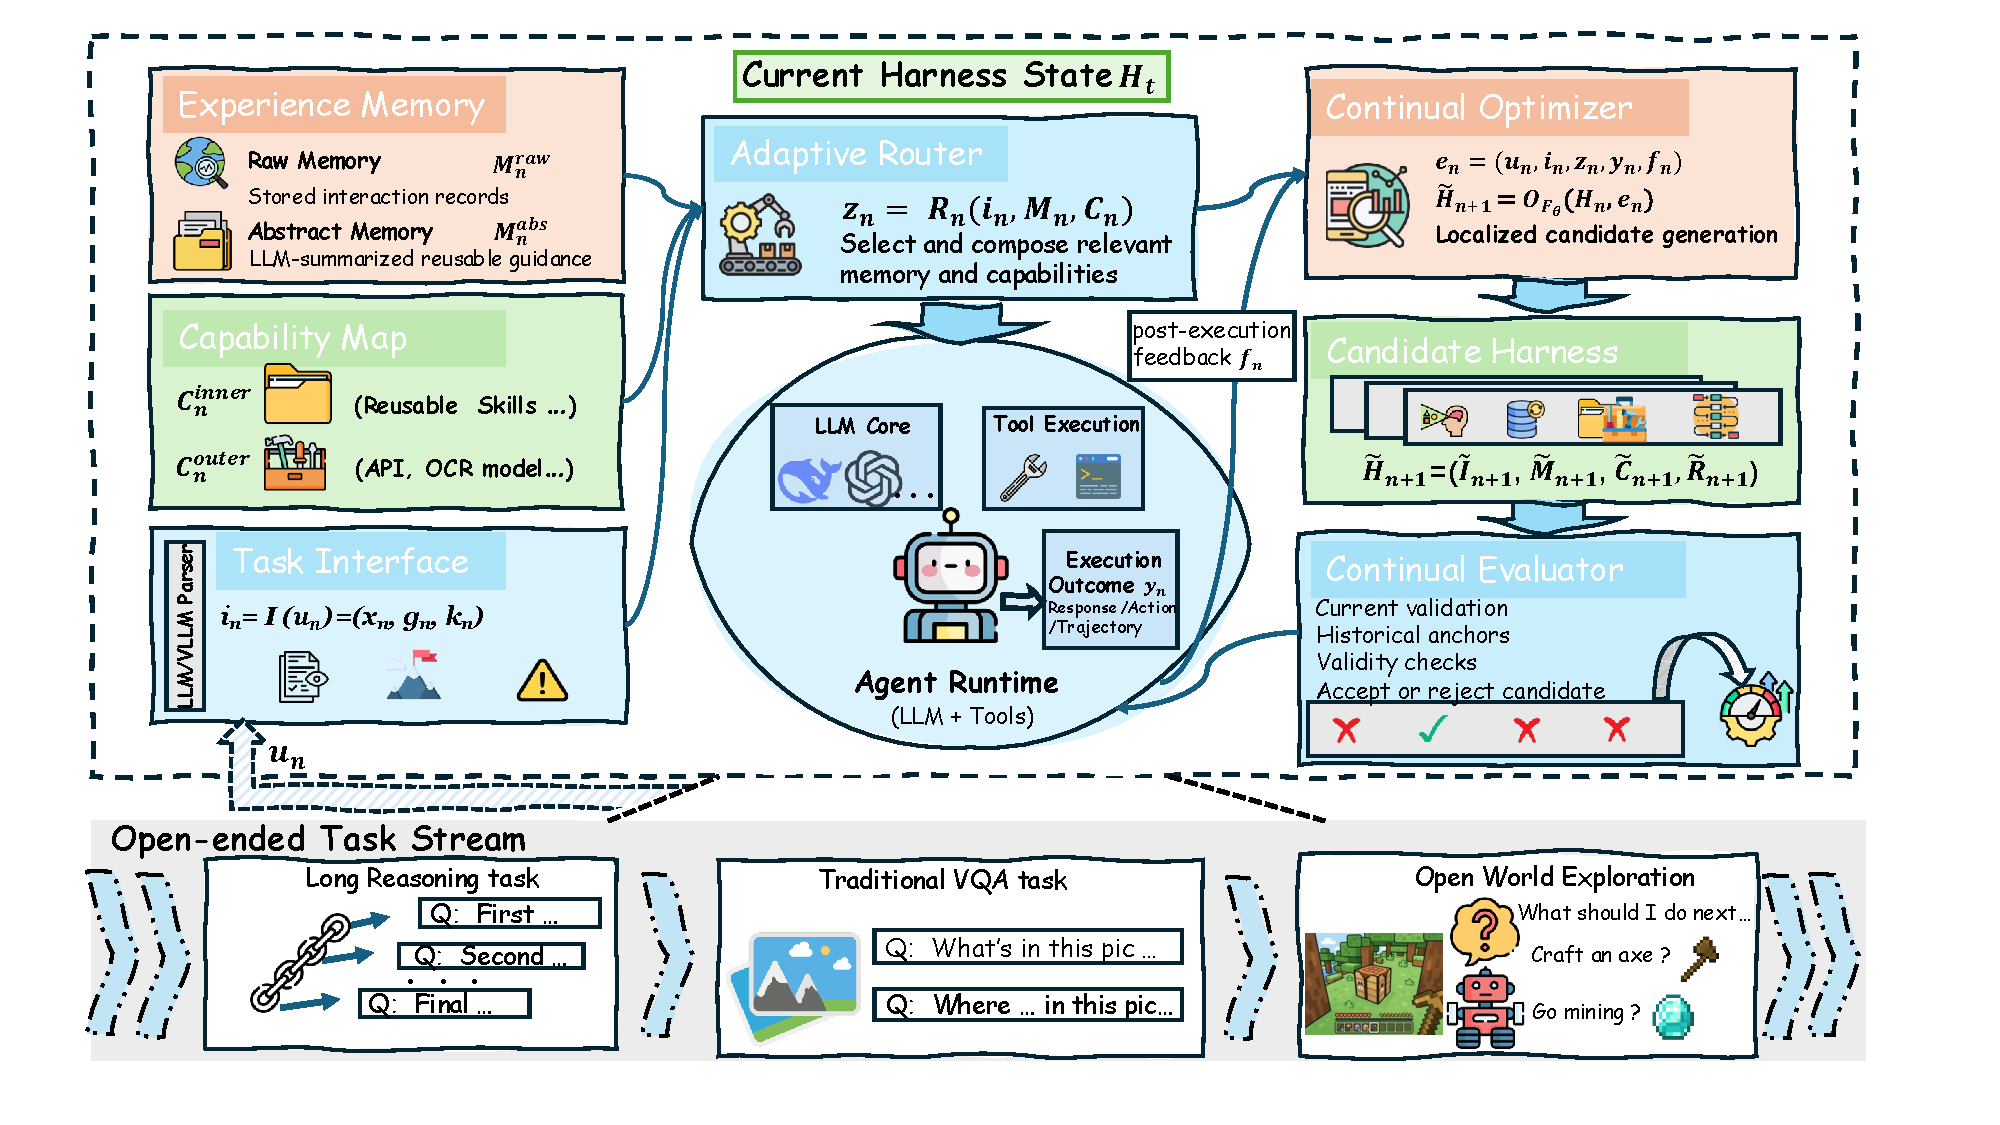
\includegraphics[width=\linewidth]{Figures/framework.pdf}
\caption{
Overview of the HCL framework. The deployed harness $H_n$ supports the
execution path from raw interaction $\mathbf{u}_n$ to outcome
$\mathbf{y}_n$. When post-execution feedback is available, the Continual
Optimizer proposes a candidate harness $\widetilde{H}_{n+1}$, and the Continual Evaluator accepts or rejects it based on current improvement, historical retention, and validity. }
\label{fig:hcl_framework}
\end{figure*}

\subsubsection{Task Interface}
\label{sec:task_interface}

The Task Interface is the input-processing layer of the harness. It transforms
a raw task interaction $\mathbf{u}_n$ into a structured representation of the
available input, task objective, and execution constraints:
\begin{equation}
\label{eq:task_interface}
\mathbf{i}_n
=
I_n\left(\mathbf{u}_n\right)
=
\left(
\mathbf{x}_n,
\mathbf{g}_n,
\mathbf{k}_n
\right),
\end{equation}
where $\mathbf{x}_n$ contains the available input,
$\mathbf{g}_n$ specifies what the task aims to accomplish, and
$\mathbf{k}_n$ records constraints such as output format, legal tool use, and
environment restrictions. Internally, $I_n$ specifies the prompts, task
templates, and parsing and normalization rules used by an LLM-based parser to
perform this transformation.

In HCL, the Task Interface maps heterogeneous task data into a unified
representation, making the relevant input, objective, and constraints explicit.
This helps the agent focus on task requirements and process different task
forms within the same continual learning pipeline. Since interface updates may
change how tasks are interpreted, $I_n$ is versioned with the harness.

\subsubsection{Experience Memory}
\label{sec:experience_memory}

Agent memory can take many forms, including episodic records, summaries, and
reflections
\citep{
park2023generativeagentsinteractivesimulacra,
packer2024memgptllmsoperatingsystems,
zhong2024memorybank,
shinn2023reflexion,
wang2024agentworkflowmemory}. From a continual learning perspective, HCL
organizes accumulated experience into two complementary forms:
\begin{equation}
\label{eq:experience_memory}
M_n
=
\left(
M_n^{\mathrm{raw}},
M_n^{\mathrm{abs}}
\right),
\end{equation}
where $M_n^{\mathrm{raw}}$ and $M_n^{\mathrm{abs}}$ denote Raw Memory and
Abstract Memory, respectively. Raw Memory preserves concrete interactions,
whereas Abstract Memory extracts reusable knowledge from them.

Raw Memory $M_n^{\mathrm{raw}}$ stores the raw task input $\mathbf{u}_n$, the
resulting response or action trajectory $\mathbf{y}_n$, and the subsequent
environment or verifier feedback $\mathbf{f}_n$. To keep memory collection
simple and storage bounded, it retains a fixed number of interactions from each
task in arrival order. These records preserve task-specific evidence about
successful behavior and encountered failures, helping the agent reuse earlier
solutions and avoid repeating previous errors.

Abstract Memory $M_n^{\mathrm{abs}}$ is produced by using an LLM to summarize
the contents of Raw Memory. The LLM consolidates recurring patterns into scoped
guidance, such as output conventions, reliable reasoning patterns, and common
errors to avoid. 
As new raw interactions are
stored, the summarization process can produce new or updated abstract entries
for related future tasks.

Raw Memory retains concrete experience for replay and behavioral recovery,
while Abstract Memory generalizes that experience for transfer across tasks.
Together, they support adaptation to new tasks while preserving useful
knowledge acquired earlier.
\subsubsection{Capability Map}
\label{sec:capability_map}

The Capability Map defines the operations and skills that the agent can invoke
during execution. HCL organizes these capabilities by their origin:
\begin{equation}
\label{eq:capability_map}
C_n
=
\left(
C_n^{\mathrm{outer}},
C_n^{\mathrm{inner}}
\right),
\end{equation}
where $C_n^{\mathrm{outer}}$ contains capabilities provided by the external
runtime, and $C_n^{\mathrm{inner}}$ contains skills acquired through continual
interaction.

Outer capabilities connect the frozen model to external resources, such as
APIs, retrieval services, perception models, calculators, and environment
actions. Each entry specifies its function, expected inputs and outputs,
invocation protocol, availability conditions, and known limitations. These
capabilities provide the basic operations needed to access information and act
in different environments.

Inner capabilities are reusable skills further abstracted from
$M_n^{\mathrm{abs}}$. An LLM can consolidate related abstract memories into
more general skills with explicit inputs, outputs, execution steps, and
applicable scopes. This turns knowledge accumulated from earlier interactions
into procedures that can be directly invoked across tasks. As Abstract Memory
evolves, new inner skills can be added and existing skills can be revised.

Unlike a static capability map limited to a predefined library of external
operations, $C_n$ can expand its executable skill set through experience. This
dynamic connection between accumulated knowledge and inner capabilities allows
the frozen-model agent to continually acquire, refine, and transfer skills
across tasks.
\subsubsection{Adaptive Router}
\label{sec:adaptive_router}

The Adaptive Router connects the Task Interface, Experience Memory, and
Capability Map to task execution. Given the structured interaction
$\mathbf{i}_n$, it retrieves relevant experience from $M_n$, selects
capabilities from $C_n$, and organizes them into an execution context:
\begin{equation}
\label{eq:adaptive_router_context}
\mathbf{z}_n
=
R_n
\left(
\mathbf{i}_n,
M_n,
C_n
\right).
\end{equation}
The resulting $\mathbf{z}_n$ contains the structured task representation,
selected experience and capabilities, and the workflow used for execution.

As $M_n$ and $C_n$ evolve, which experience and capabilities are useful for a
task and how they should be organized may also change. At each interaction,
$R_n$ uses an LLM together with its routing prompts, selection criteria, and
workflow templates to adapt the execution strategy to the current task and
available contents. These routing specifications can also be revised across
interactions, allowing the Router to evolve alongside Memory and the Capability
Map. The frozen model and external runtime then use $\mathbf{z}_n$ to produce
the response or action $\mathbf{y}_n$.

\subsection{Guarded Harness Evolution}
\label{sec:guarded_evolution}

A harness update may improve current behavior while degrading previously
reliable behavior on earlier tasks. We therefore introduce \emph{guarded
harness evolution}, which separates update generation from deployment through
a proposal--evaluation--commitment process. Given feedback, the Continual Optimizer
produces an isolated candidate harness. The Continual Evaluator commits it only if it satisfies current-improvement, historical-retention, and validity requirements. Otherwise, $H_n$ remains deployed. This process makes retention an explicit condition for harness evolution rather than assuming that a useful update on the current task is safe for earlier tasks.

\subsubsection{Continual Optimizer: Candidate Generation}
\label{sec:continual_optimizer}

Interaction feedback indicates whether the current execution is successful, but
does not specify how the harness should change. The Continual
Optimizer implements the update operator $\mathcal{O}$ in
Eq.~(\ref{eq:hcl_candidate_transition}) using a prompt template for the
foundation model $F_\theta$. It provides the deployed harness $H_n$ and the
interaction evidence $\mathbf{e}_n$ to the model and asks it to propose a
candidate harness $\widetilde{H}_{n+1}$.
$F_\theta$ analyzes the execution outcome in light of the feedback and examines the execution context to identify which harness components require revision. It may modify prompts or parsing rules in the Task Interface, record or summarize experience in Memory, add or revise skills in the Capability Map, or adjust selection and workflow rules in the Adaptive Router.


To provide alternative update directions while limiting repeated LLM calls, we
use a simple sequential strategy when multiple components require revision. The
selected components are considered in a predefined order. For each component,
the Optimizer generates up to $K$ alternatives one at a time. Each alternative is evaluated by replacing only the selected component in the current candidate harness while keeping all other components fixed. For each selected component, the Continual Optimizer generates up to K alternatives, each of which is evaluated while all other components remain fixed. The highest-scoring admissible alternative is retained as the basis for revising the next component. If no alternative passes the gate, that component remains unchanged. The deployed harness
$H_n$ remains unchanged until the resulting candidate completes evaluation and
is committed.


\subsubsection{Continual Evaluator: Historical Evaluation and Commitment}
\label{sec:continual_evaluator}

To align harness updates with the objective of continual learning, we
introduce a retention-aware evaluation standard rather than judging candidates
only by current-task gains. The Continual Evaluator $E$ examines three
complementary aspects: \emph{current improvement} measures whether the candidate
better solves the current task, \emph{historical retention} checks whether
previously reliable behavior is preserved, and \emph{validity} ensures that the
updated harness and its outputs remain usable. The deployed harness $H_n$ and
candidate $\widetilde{H}_{n+1}$ are evaluated under the same model, decoding,
tool, environment, and seed conditions to provide a controlled comparison. A
candidate can replace $H_n$ only when all three requirements are satisfied,
allowing the harness to acquire new behavior without ignoring what it has
already learned.

\paragraph{Current Improvement.}
Let $V_n$ denote the validation cases for the current task, and let
$P(H,V_n)$ denote the performance of harness $H$ on these cases. The improvement
produced by the candidate is
\begin{equation}
\label{eq:evaluator_validation}
\Delta_n
=
P\left(\widetilde{H}_{n+1},V_n\right)
-
P\left(H_n,V_n\right).
\end{equation}
The candidate satisfies this criterion when
$\Delta_n \geq \delta_n$, where $\delta_n$ is the predefined minimum
improvement. Depending on the task, $P$ may measure answer accuracy, tool-use
success, or environment completion.

\paragraph{Historical Retention.}
Current-task improvement does not indicate whether a candidate preserves behavior acquired earlier. The Evaluator therefore maintains a compact anchor set $A_n$ for historical evaluation. Each anchor contains the raw input and success criterion of a previously observed case, allowing that case to be rerun under both the deployed and candidate harnesses. At the end of each task, anchors are selected using a predefined ratio of previously successful and failed cases. If either group contains too few cases to meet its target, the remaining slots are filled from the other group. The anchors are used only for evaluation and are unavailable during candidate generation. For each anchor $a\in A_n$, define the binary success indicator
\begin{equation}
\label{eq:anchor_success}
q(H,a)\in\{0,1\},
\end{equation}
where $q(H,a)=1$ if harness $H$ satisfies the corresponding success criterion and 0 otherwise.
The historical loss introduced by the candidate is
\begin{equation}
\label{eq:evaluator_historical_loss}
D_n
=
\sum_{a\in A_n}
\mathbf{1}
\left[
q(H_n,a)=1
\land
q\left(\widetilde{H}_{n+1},a\right)=0
\right],
\end{equation}

where $\mathbf{1}[\cdot]$ is the indicator function, equal to 1 when the enclosed condition holds and 0 otherwise.

Therefore, $D_n$ counts previously solved anchors that fail under the candidate.
The candidate satisfies the historical-retention criterion when $D_n \leq B_n$, where $B_n$ is the predefined tolerance for historical loss.
Setting $B_n=0$ requires the candidate to preserve every anchor currently solved by $H_n$. Appendix~\ref{app:anchor_criteria} specifies the success criterion $q(H,a)$ used for each experimental task.

\paragraph{Validity Check.}
The candidate must also be executable and comply with the task and runtime
requirements. Let $\mathcal{L}_n$ denote the set of validity checks applied at
interaction step $n$. For each $\ell \in \mathcal{L}_n$, define
\begin{equation}
\label{eq:evaluator_validity}
v_{n,\ell}\left(\widetilde{H}_{n+1}\right)\in\{0,1\},
\end{equation}
where $v_{n,\ell}\left(\widetilde{H}_{n+1}\right)=1$ indicates that the
candidate satisfies validity check $\ell$, and $0$ otherwise. These checks may
cover artifact syntax, output-schema compliance, legal tool use, task
constraints, and environment consistency.

The three criteria are combined into a candidate-specific commitment
decision:
\begin{equation}
\label{eq:evaluator_decision}
G_n^{(k)}
=
\mathbf{1}
\left[
(\Delta_n^{(k)} \geq \delta_n)
\land
(D_n^{(k)} \leq B_n)
\land
\left(
\forall \ell,\;
v_{n,\ell}\left(\widetilde{H}_{n+1}^{(k)}\right)=1
\right)
\right].
\end{equation}
The decision rule in Eq.~(\ref{eq:evaluator_decision}) serves as a hard admissibility gate. When multiple candidates pass the gate, the Continual Evaluator ranks them using a composite score that aggregates their current-performance, validity, and historical-retention scores. The highest-scoring candidate is committed as $H_{n+1}$, with ties broken randomly. If no candidate passes the gate, $H_n$ remains deployed.

By making historical retention a necessary condition for commitment, the
admissibility gate supports the acquisition of new behavior while explicitly
controlling the loss of previously reliable behavior. The tolerance $B_n$
further adjusts the balance between stability and plasticity.

\subsection{Connections to Model-Centric Continual Learning}
\label{sec:hcl_model_cl}

HCL draws on several complementary principles from model-centric continual learning,
but realizes them through harness mechanisms rather than model-parameter
updates \citep{delange2021continual,wang2024comprehensive}. Replay-based methods
retain earlier examples to preserve acquired knowledge. Experience Memory
follows this principle by storing concrete interactions for later reuse.
Representation-based methods learn abstractions that support transfer across
tasks. The Capability Map similarly transforms accumulated experience into
reusable skills and combines them with external capabilities. Architecture-based
methods organize reusable modules and routines to reduce interference. HCL
represents these routines as invocable capabilities and uses the Adaptive
Router to select and compose them for each interaction. Optimization- and regularization-based
methods control parameter updates using information from
earlier tasks, allowing new knowledge to be acquired while limiting interference
with previous knowledge. 
HCL applies the same principle to harness updates
through the Continual Optimizer and Continual Evaluator. 
The Optimizer proposes
candidate changes from current feedback, while the Evaluator tests them on
current validation cases and historical anchors. 
Only candidates that improve
current performance while satisfying historical retention and validity
requirements are committed.
This proposal--evaluation--commitment process integrates adaptation and protection into continual harness evolution.

These relationships are conceptual rather than one-to-one implementations.
More importantly, \textit{HCL brings the complementary principles of model-centric
continual learning into a unified system-level formulation}. Traditional
approaches \citep{kang2025dynamic,liu2026branch} often treat replay, representation, architecture, optimization, and
regularization as separate solution families for adapting model parameters.
HCL coordinates their functions within a single evolving harness under the
same acquisition--retention objective. It therefore extends continual learning
from parameter adaptation to the coordinated evolution of agent
infrastructure, providing a unified framework for continual learning beyond
the model itself.
\section{Experiments}
\label{sec:experiments}

We evaluate HCL in two regimes. ALFWorld \citep{alfworld} and Minecraft \citep{voyager} examine capability accumulation, reuse, and failure recovery during open-world interaction.
Textual reasoning and multimodal perception use controlled task streams with
repeated evaluation of previously observed tasks, making harness-level
forgetting and the stability--plasticity trade-off directly measurable. We
also evaluate the control of this trade-off and ablate the four editable
harness components.
We use different foundation models across the experimental settings to examine
whether HCL generalizes across model families and scales rather than depending
on a particular model. ALFWorld uses Qwen3.5-9B; Minecraft and the main
multimodal experiments use Qwen3.6-27B; textual reasoning uses
DeepSeek-V4-Flash; and the component ablation uses Qwen3.5-4B. Within each
setting, the same foundation model is used for all comparisons and remains
frozen throughout the continual-learning stream. Any adaptation therefore
comes from harness updates rather than model training.

\subsection{Evaluation Protocol}
\label{sec:experimental_setup}

For each task stream, a single harness evolves sequentially around the same
foundation model. Let $H^{(s)}$ denote the deployed harness after learning task
$\mathcal{D}_s$, where $s$ indexes the evaluation stage. At the end of each
stage, we evaluate $H^{(s)}$ on the current task and every previously observed
task:
\begin{equation}
\label{eq:exp_performance}
R_{s,j}
=
\operatorname{Eval}
\left(
H^{(s)},
\mathcal{D}^{\mathrm{test}}_j
\right),
\qquad
j \leq s,
\end{equation}
where $R_{s,j}$ is the benchmark score or episode success rate on task $j$.
Current-task validation cases and historical anchors are used only by the
Continual Evaluator to determine whether a candidate can be committed. The
final test sets are disjoint from both and are used only for reporting.

For task streams with metrics on a common scale, we report final average
performance and average old-task forgetting:
\begin{equation}
\label{eq:exp_metrics}
\operatorname{Avg}_T
=
\frac{1}{T}
\sum_{j=1}^{T}
R_{T,j},
\qquad
\operatorname{Fgt}_T
=
\frac{1}{T-1}
\sum_{j=1}^{T-1}
\left(
\max_{r\in\{j,\ldots,T\}}
R_{r,j}
-
R_{T,j}
\right).
\end{equation}
$\operatorname{Avg}_T$ measures final performance across the complete stream,
while $\operatorname{Fgt}_T$ measures the average decline of earlier tasks
from their best observed performance. Forgetting is marked as ``--''
for Zero-shot and Static Harness because they make no sequential updates.

Stability-HCL and Plasticity-HCL are two configurations of the framework, differing only in the historical-loss tolerance $B_n$. Stability-HCL sets
$B_n=0$ and rejects any candidate that causes a currently solved anchor to
fail. Plasticity-HCL sets $B_n=\infty$, so historical anchor losses do not
block a candidate as long as it satisfies the current-improvement and validity
requirements. We evaluate both
configurations in ALFWorld and the controlled streams, while Minecraft uses
the retention-oriented configuration. Detailed settings are provided in
Appendix~\ref{app:implementation}.
\subsection{Open-World Capability Accumulation}
\label{sec:open_world_experiments}

We study long-horizon harness evolution in ALFWorld and
Minecraft. ALFWorld supports stage-wise evaluation across
previously observed task categories, while Minecraft provides a longer
interaction curriculum for examining capability accumulation, failure
recovery, and skill revision.

\subsubsection{ALFWorld}
\label{sec:alfworld_experiment}

We use the text-based ALFWorld environment with a maximum of 50 interaction
steps per episode. The continual stream contains six task categories in the
order of Pick-and-Place, Look-in-Light, Clean, Heat, Cool, and Two-object
manipulation. For each category, 10 training episodes are used for sequential
adaptation. After each stage, the harness is evaluated on all observed
categories, with final performance reported on the 134 official evaluation
episodes.

\begin{table}[t]
    \centering
    \caption{
        Final performance and harness-level forgetting on ALFWorld with
        Qwen3.5-9B as the frozen foundation model.
        The best and second-best results in each metric column are marked in
        bold and underlined, respectively.
    }
    \label{tab:alfworld}
    \resizebox{\linewidth}{!}{
    \begin{tabular}{lcccccc|cc}
        \toprule
        Method
        & Pick
        & Look
        & Clean
        & Heat
        & Cool
        & Two-object
        & Final Avg. \(\uparrow\)
        & Avg. Fgt. \(\downarrow\) \\
        \midrule

        Static Harness
        & \underline{95.80}
        & 66.70
        & 25.80
        & 26.10
        & 9.50
        & 58.80
        & 47.12
        & -- \\

        RAG Baseline
        & \underline{95.80}
        & \textbf{83.30}
        & 41.90
        & \underline{39.10}
        & 14.30
        & 58.80
        & 55.56
        & \textbf{1.74} \\

        MemP \citep{memp}
        & \underline{95.80}
        & \textbf{83.30}
        & \underline{48.40}
        & 34.80
        & 9.50
        & 47.10
        & 53.15
        & 5.18 \\

        MemRL \citep{zhang2026memrl}
        & 87.50
        & 66.70
        & 29.00
        & \textbf{60.90}
        & \underline{23.80}
        & 41.20
        & 51.51
        & 5.64 \\

        Stability-HCL (Ours)
        & \textbf{100.00}
        & \textbf{83.30}
        & \textbf{51.60}
        & 30.40
        & \textbf{28.60}
        & \underline{76.50}
        & \underline{61.74}
        & \underline{2.64} \\

        Plasticity-HCL (Ours)
        & \textbf{100.00}
        & \underline{77.80}
        & 41.90
        & \underline{39.10}
        & 19.00
        & \textbf{100.00}
        & \textbf{62.98}
        & 10.94 \\

        \bottomrule
    \end{tabular}
    }
\end{table}
We compare HCL with a Static Harness, a RAG baseline, MemP \citep{memp}, and MemRL \citep{zhang2026memrl}. 
For fairness, MemP and MemRL are reimplemented within our framework with unified data processing and action selection, while their algorithms remain unchanged.
Table~\ref{tab:alfworld} shows that reusing past experience improves the Static
Harness but is insufficient for broad continual adaptation. RAG increases the
final average from 47.12\% to 55.56\% and achieves the lowest average
forgetting among the adaptive baselines. However, retrieval alone cannot revise
reusable procedures or routing rules. MemP and MemRL also improve individual
categories, but their performance varies considerably across the
stream. These results show that memory-based adaptation supports experience
reuse, but does not consistently balance capability acquisition and retention.

Both HCL profiles achieve stronger overall performance by evolving the complete
harness. Plasticity-HCL obtains the highest final average of 62.98\% and
solves all Two-object episodes, showing the strongest adaptation to the latest
task but also greater forgetting. Stability-HCL reaches a comparable 61.74\%
and performs best on four of the six categories while substantially reducing
average forgetting. Plasticity-HCL therefore favors capability
acquisition, whereas Stability-HCL provides a better balance between adaptation
and retention. Since the foundation model is frozen and the two profiles differ
only in $B_n$, this comparison shows that the Continual Evaluator can
explicitly control the stability--plasticity trade-off.




\subsubsection{Minecraft}
\label{sec:minecraft_experiment}

We evaluate HCL with Qwen3.6-27B on a 50-task Minecraft curriculum that spans
resource collection, crafting, mining, tool use, object placement, smelting,
and tasks with multiple dependent operations. 
After each interaction, environment feedback is
stored in Experience Memory and can be used to refine reusable capabilities
and execution workflows. Previously validated skill tests are retained as
historical anchors. A capability addition or revision is committed only when
it improves the current objective and continues to pass all applicable retained
tests. For comparison, the Static Harness follows the same curriculum without
evolution. MemRL and MemP are reproduced within our harness as memory-management
baselines, rather than run from their official repositories.

\begin{figure*}[t]
    \centering
    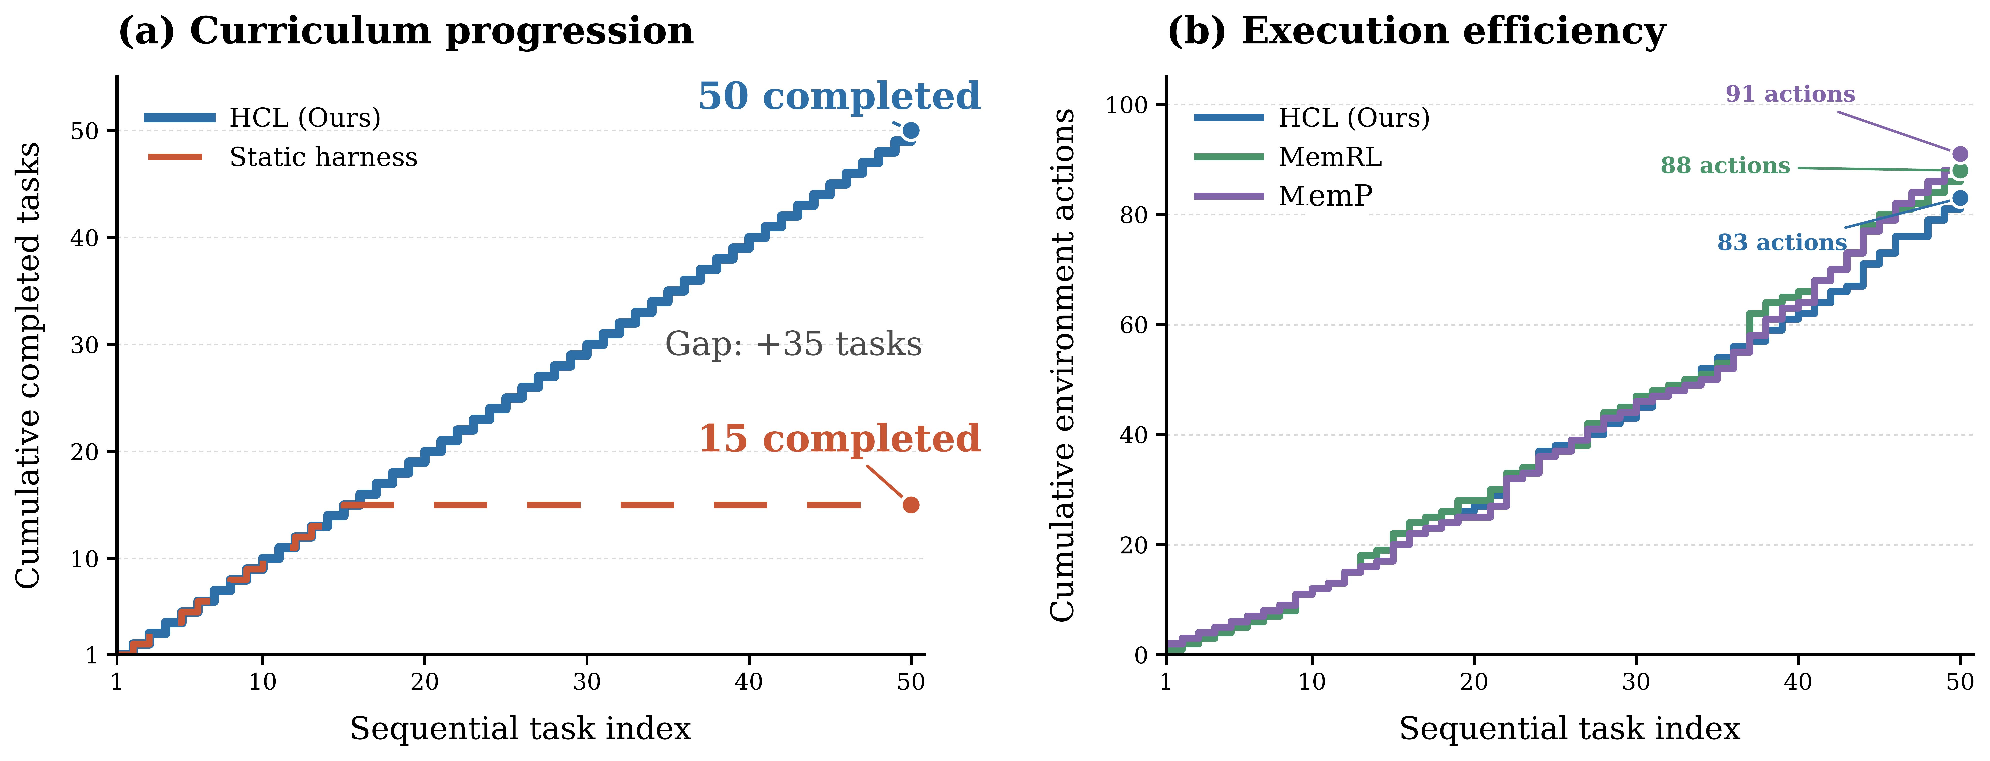
\includegraphics[width=\textwidth]
    {Figures/curriculum_comparison.pdf}
    \caption{
        Curriculum progression and execution efficiency.
        \textbf{(a)} HCL completes all 50 tasks, while the Static Harness
        plateaus at 15. \textbf{(b)} Cumulative environment actions over the
        50-task curriculum: HCL uses 83, versus 88 for MemRL and 91 for MemP;
        lower is more efficient.
    }
    \label{fig:minecraft_evolution}
\end{figure*}

Figure~\ref{fig:minecraft_evolution} shows differences in progression and
execution efficiency. The Static Harness follows HCL for 15 tasks and then
plateaus; HCL completes all 50, progressing from collection and crafting to
persistent assets and coordinated multi-step execution. HCL uses 83 environment
actions, compared with 88 for MemRL and 91 for MemP, indicating less redundant
execution. Across later multi-step tasks, HCL avoids repeated diagnosis,
crafting, and recovery actions, so its lower curve reflects more efficient
reuse of accumulated experience while retaining progression across the full
curriculum. Reproducing both baselines in our harness keeps the task interface,
capability library, and environment stack common while varying memory
management. These results show that HCL supports efficient continual adaptation
without updating the foundation model.


\subsection{Controlled Harness Continual Learning}
\label{sec:controlled_tasks}

We next evaluate HCL on task sequences. Within each stream, all HCL profiles
share the same foundation model, task order, data allocation, editable
artifacts, and candidate generator.

\subsubsection{Textual Reasoning}
\label{sec:textual_reasoning_experiment}

The textual stream follows the order MuSiQue
\citep{trivedi-etal-2022-musique}, ProofWriter
\citep{tafjord-etal-2021-proofwriter}, GSM8K
\citep{cobbe2021trainingverifierssolvemath}, and HotpotQA
\citep{yang-etal-2018-hotpotqa}. These tasks cover multi-hop question
answering, logical deduction, mathematical reasoning, and
knowledge-intensive question answering. For each task, we use 250 examples
for adaptation, 50 for validation, and 500 for testing. The foundation model
remains frozen throughout the stream. HCL updates only the Task Interface,
Experience Memory, Capability Map, and Adaptive Router.

\begin{table}[t]
    \centering
    \caption{
    Final performance after the four-task textual-reasoning stream with
    DeepSeek-V4-Flash as the frozen foundation model. The Zero-shot baseline
    evaluates each task independently without sequential harness updates.
     The best and second-best results in each metric
    column are marked in bold and underlined, respectively.
    }
    \label{tab:text_main_results}
    \resizebox{\linewidth}{!}{
    \begin{tabular}{lcccc|cc}
        \toprule
        Method
        & MuSiQue
        & ProofWriter
        & GSM8K
        & HotpotQA
        & Final Avg. $\uparrow$
        & Avg. Fgt. $\downarrow$ \\
        \midrule

        DeepSeek-V4-Flash Zero-shot
        & \textbf{35.00}
        & 42.80
        & 49.40
        & 54.80
        & 45.50
        & -- \\

        \textbf{Stability-HCL (Ours)}
        & 27.60
        & \underline{73.00}
        & \underline{50.40}
        & \underline{57.80}
        & \underline{52.20}
        & \textbf{0.00} \\

        \textbf{Plasticity-HCL (Ours)}
        & \underline{29.00}
        & \textbf{77.00}
        & \textbf{92.00}
        & \textbf{60.80}
        & \textbf{64.70}
        & \underline{0.07} \\
        \bottomrule
    \end{tabular}
    }
\end{table}

Table~\ref{tab:text_main_results} shows how different historical-loss tolerances shift HCL between stronger retention and stronger adaptation. Stability-HCL requires accepted
updates to preserve performance on the historical anchor set, reducing average
forgetting to zero. This strict constraint substantially
limits adaptation, resulting in a final average of 52.20\%, compared with
64.70\% for Plasticity-HCL. Nevertheless, Stability-HCL still outperforms the
45.50\% zero-shot baseline, showing that it can acquire new behavior while
fully retaining the previously measured behavior.

Plasticity-HCL relaxes the historical-retention requirement and therefore
permits more aggressive harness updates. This increases the final average
from 52.20\% to 64.70\%, while introducing only 0.07 average forgetting.
With DeepSeek-V4-Flash frozen throughout the stream, these results show that
the Continual Evaluator can shift HCL between stronger retention and stronger
adaptation solely through the historical-loss tolerance.

\subsubsection{Multimodal Perception}
\label{sec:multimodal_experiment}

The multimodal stream follows the order of COCO object detection, COCO image
captioning, RefCOCO visual grounding, and VQAv2. Qwen3.6-27B remains frozen
throughout the stream. For each task, we use 250 examples for adaptation, 50
for validation, and 500 for testing. We additionally compare with
DGG~\citep{li2026dgg}, a recent adaptive method for sequential multi-task
continual learning whose setting aligns with this controlled multimodal stream.

\begin{table}[t]
    \centering
    \caption{
        Final performance after the four-task multimodal-perception stream with
        Qwen3.6-27B as the frozen foundation model. The Zero-shot baseline
        evaluates each task independently without sequential harness updates.
        The best and second-best results in each metric
        column are marked in bold and underlined, respectively.
    }
    \label{tab:multimodal_results}
    \resizebox{\linewidth}{!}{
        \begin{tabular}{lcccc|cc}
            \toprule
            Method
            & Detection
            & Caption
            & Grounding
            & VQAv2
            & Final Avg. $\uparrow$
            & Avg. Fgt. $\downarrow$ \\
            \midrule

            Qwen3.6-27B Zero-shot
            & 4.27
            & 25.47
            & 43.00
            & \textbf{84.87}
            & 39.40
            & -- \\

            DGG \citep{li2026dgg}
            & 29.58
            & 29.77
            & 48.96
            & 62.60
            & 42.73
            & \underline{0.26} \\

            Plasticity-HCL (Ours)
            & \underline{64.14}
            & \underline{37.31}
            & \underline{90.60}
            & \underline{79.80}
            & \underline{67.96}
            & 0.81 \\

            Stability-HCL (Ours)
            & \textbf{65.34}
            & \textbf{39.41}
            & \textbf{91.60}
            & 79.33
            & \textbf{68.92}
            & \textbf{0.22} \\

            \bottomrule
        \end{tabular}
    }
\end{table}

Table~\ref{tab:multimodal_results} shows that both HCL profiles substantially
outperform Zero-shot and DGG in final average. The largest gains occur in
detection and grounding, where the harness must organize spatial information
into task-specific outputs. HCL also improves captioning, indicating that its
evolving components can support different multimodal objectives and output
formats within one task stream.

VQAv2 is the only task on which Zero-shot remains stronger, as the frozen model
already performs well on direct image--question answering. Nevertheless, both
HCL profiles retain substantially higher VQAv2 performance than DGG.
Stability-HCL achieves the highest final average of 68.92\% and the lowest
forgetting of 0.22, while Plasticity-HCL reaches a similar final average of
67.96\%. Overall, HCL enables a single frozen model to continually handle
heterogeneous multimodal tasks while maintaining a stronger
stability--plasticity balance.
\subsection{Stability--Plasticity Trade-off}
\label{sec:stability_plasticity}

Following Eq.~(\ref{eq:evaluator_decision}), we vary only the historical-loss tolerance $B_n$ in $D_n \leq B_n$, while holding the current-improvement and validity criteria fixed. Specifically, $\delta_n$ in Eq.~(\ref{eq:evaluator_validation}) requires an improvement of at least two correct validation cases. Under the validity criterion in Eq.~(\ref{eq:evaluator_validity}), each candidate must achieve at least 90.00\% output-format compliance and introduce no syntax, tool-use, or environment violations. These thresholds are chosen heuristically to balance current-task improvement with candidate reliability and remain identical across all settings.

The historical loss $D_n$ in
Eq.~(\ref{eq:evaluator_historical_loss}) counts anchors that are solved by
$H_n$ but fail under $\widetilde{H}_{n+1}$. Within each run, we fix
$B_n \equiv b$ for all candidate decisions and compare
$b \in \{0,1,3,\infty\}$. The settings $b=0$ and $b=\infty$ correspond to
Stability-HCL and Plasticity-HCL, respectively. The intermediate settings
$b=1$ and $b=3$ allow each candidate to introduce at most one and three newly
failed anchors across $A_n$. Each run uses 300 adaptation, 80 validation, and 600 test examples per task, with 80 anchors for every earlier task. A predefined parameter controls the composition of previously successful and failed examples in each anchor set. If either group contains too few examples to meet its target, the remaining slots are filled from the other group. All other experimental conditions remain fixed.

\begin{table}[t]
    \centering
    \caption{
        Performance under different fixed values of $b$, where
        $B_n \equiv b$ within each run. All other experimental conditions
        are held constant. The best and second-best results in each metric
        column are marked in bold and underlined, respectively.
    }
    \label{tab:text_threshold}
    \resizebox{\linewidth}{!}{
        \begin{tabular}{lcccc|cc}
            \toprule
            Historical-loss tolerance $b$
            & MuSiQue
            & ProofWriter
            & GSM8K
            & HotpotQA
            & Final Avg. $\uparrow$
            & Avg. Fgt. $\downarrow$ \\
            \midrule

            $b=0$
            & \underline{27.83}
            & 73.33
            & \underline{84.33}
            & \textbf{59.50}
            & 61.25
            & \textbf{0.39} \\

            $b=1$
            & 24.83
            & \underline{77.50}
            & \textbf{92.33}
            & \underline{59.17}
            & \textbf{63.46}
            & \underline{1.22} \\

            $b=3$
            & 26.83
            & \textbf{79.83}
            & 83.00
            & 58.50
            & \underline{62.04}
            & 2.00 \\

            $b=\infty$
            & \textbf{28.33}
            & 71.00
            & 82.00
            & \underline{59.17}
            & 60.13
            & 3.45 \\

            \bottomrule
        \end{tabular}
    }
\end{table}

\begin{figure*}[t]
    \centering
    \begin{subfigure}[t]{0.49\textwidth}
        \centering
        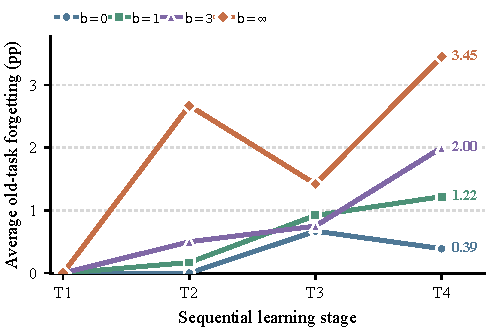
\includegraphics[width=\linewidth]
        {Figures/textual_forgetting_trajectory_styled.pdf}
        \caption{
            Textual reasoning under different fixed values of $b$.
        }
        \label{fig:textual_forgetting}
    \end{subfigure}
    \hfill
    \begin{subfigure}[t]{0.49\textwidth}
        \centering
        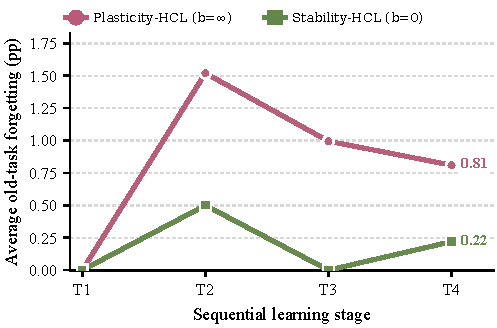
\includegraphics[width=\linewidth]
        {Figures/multimodal_forgetting_trajectory_styled.pdf}
        \caption{
            Multimodal perception under $b=0$ and $b=\infty$.
        }
        \label{fig:multimodal_forgetting}
    \end{subfigure}
    \caption{
        Stage-wise forgetting under different fixed historical-loss
        tolerances.
    }
    \label{fig:controlled_forgetting}
\end{figure*}

Table~\ref{tab:text_threshold} shows that increasing $b$ weakens retention.
Average forgetting rises from 0.39 at $b=0$ to 3.45 at $b=\infty$. Final
performance does not increase accordingly: the highest final average of
63.46\% occurs at $b=1$, while the unrestricted setting reaches 60.13\%. One possible explanation is that each committed update changes the subsequent evolution trajectory: without historical constraints, locally beneficial updates may overwrite reusable harness contents, weakening both retention and the experience or capabilities available for later tasks. 
A moderate value of $b$ therefore provides additional flexibility for
adaptation without allowing excessive historical loss. The remaining
forgetting at $b=0$ occurs because the constraint covers a finite anchor set,
whereas forgetting is evaluated on separate historical test cases. Preserving
all anchors currently solved by $H_n$ cannot guarantee unchanged behavior on
historical cases not represented by $A_n$.


Figure~\ref{fig:controlled_forgetting} complements these final results by showing how forgetting develops across the task sequence. In the textual stream shown in Figure~\ref{fig:controlled_forgetting}(a), smaller values of $b$ generally maintain lower forgetting, with final forgetting increasing consistently from 0.39 at $b=0$ to 3.45 at $b=\infty$. In the multimodal stream shown in Figure~\ref{fig:controlled_forgetting}(b), Stability-HCL remains below Plasticity-HCL at every stage after $T_1$ and finishes with forgetting of 0.22 rather than 0.81. This pattern reflects the role of $b$ in the commitment gate: smaller values reject more candidates that improve the current task at the expense of historical behavior, thereby constraining the harness to more retention-preserving update trajectories. Larger values permit greater adaptation flexibility but expose earlier tasks to more regression. Together, the two trajectories illustrate that a stricter historical-loss tolerance suppresses forgetting throughout harness evolution.

\subsection{Ablation Study}
\label{sec:component_ablation}

We conduct component ablations on the controlled multimodal stream using
Qwen3.5-4B with the balanced HCL configuration. The stream follows COCO object detection $\rightarrow$ COCO image captioning $\rightarrow$ RefCOCO visual grounding $\rightarrow$ VQAv2, with 250 adaptation, 50 validation, and 500 test examples for each task. Starting
from Full HCL, we disable updates to one harness component at a time while
keeping the other three components adaptive. All variants use the same
foundation model, task order, evaluation criteria, and update schedule.
Table~\ref{tab:component_ablation} summarizes the resulting component-wise
ablation results.

\begin{table}[t]
    \centering
    \caption{
        Component ablation on the controlled multimodal stream.
        $I$, $M$, $C$, and $R$ denote the Task Interface, Experience Memory,
        Capability Map, and Adaptive Router. A check mark indicates that the
        component is updated, while a cross indicates that its update is
        disabled. The best and second-best results in each metric column are
        marked in bold and underlined, respectively.
    }
    \label{tab:component_ablation}
        \begin{tabular}{lcccc|cc}
            \toprule
            Component
            & $I$
            & $M$
            & $C$
            & $R$
            & Final Avg. $\uparrow$
            & Avg. Fgt. $\downarrow$ \\
            \midrule

            Zero-shot
            & -- & -- & -- & --
            & 34.84
            & -- \\

            w/o Interface update
            & $\times$ & $\checkmark$ & $\checkmark$ & $\checkmark$
            & 62.37
            & \underline{0.11} \\

            w/o Memory update
            & $\checkmark$ & $\times$ & $\checkmark$ & $\checkmark$
            & 62.28
            & 0.83 \\

            w/o Capability update
            & $\checkmark$ & $\checkmark$ & $\times$ & $\checkmark$
            & \underline{63.12}
            & \textbf{0.06} \\

            w/o Router update
            & $\checkmark$ & $\checkmark$ & $\checkmark$ & $\times$
            & 62.77
            & 0.14 \\

            Full HCL
            & $\checkmark$ & $\checkmark$ & $\checkmark$ & $\checkmark$
            & \textbf{63.41}
            & 0.45 \\

            \bottomrule
        \end{tabular}
\end{table}

Full HCL achieves the highest final average of 63.41\%, showing that the four
components contribute complementarily to continual adaptation. Disabling
Experience Memory or the Task Interface produces the largest decrease in final
performance. In particular, removing Memory updates also increases forgetting
to 0.83, indicating that evolving memory supports both the acquisition and
retention of behavior. Disabling Capability Map or Adaptive Router updates
causes smaller but consistent performance reductions. The small effect of Capability updates may reflect that this multimodal stream relies less on reusable executable procedures than the Minecraft curriculum.

Several ablations show lower forgetting than Full HCL because restricting the
editable components also limits the extent of adaptation. Lower forgetting
alone therefore does not necessarily indicate a better evolving harness and should be considered together with final performance. Exact interventions and full per-task
results are reported in Appendix~\ref{app:component_ablation_details}.
\section{Conclusion}
\label{sec:conclusion}
We formulate Harness Continual Learning (HCL) as a new continual learning paradigm in
which the agent harness, rather than model parameters, evolves through
sequential experience. Our framework treats the mutable harness components as a
unified evolving state and separates candidate generation from evaluation and
commitment, making historical retention an explicit condition for deployment.
Experiments show that harness evolution can accumulate capabilities and recover
from failures, while also causing measurable forgetting under a frozen
foundation model. Explicitly controlling historical loss enables HCL to balance
stability and plasticity. These findings demonstrate the potential of continual learning at the harness level, while highlighting unresolved challenges in efficient retention evaluation, harness-content consolidation, and evaluation over longer interaction streams. We hope HCL provides a foundation for addressing these challenges and
encourages broader research on reliable agent continual learning.

\bibliography{main}
\bibliographystyle{main}


\section*{Supplementary Material}

\appendix

The supplementary material provides implementation details, full ablation
results, and task-specific anchor criteria.

\section{Implementation and Experimental Settings}
\label{app:implementation}

\subsection{Harness and Evaluator Boundaries}

Table~\ref{tab:state_access_boundaries} summarizes the access and update
boundaries of the harness components and the evaluation-only anchor set.

\begin{table}[H]
\centering
\small
\caption{Access and update boundaries of the deployed harness and anchor set.}
\label{tab:state_access_boundaries}
\setlength{\tabcolsep}{4pt}
\begin{tabular}{
>{\raggedright\arraybackslash}p{0.20\textwidth}
>{\raggedright\arraybackslash}p{0.40\textwidth}
>{\raggedright\arraybackslash}p{0.30\textwidth}}
\toprule
Artifact & Execution and candidate-generation access & Update boundary \\
\midrule
Task Interface $I_n$
& Constructs $\mathbf{i}_n$; the Optimizer may revise prompts, templates, and
parsing or normalization rules.
& Changes enter $H_n$ only with a committed candidate. \\

Raw and Abstract Memory $M_n^{\mathrm{raw}},M_n^{\mathrm{abs}}$
& Supplies records and guidance to the Router; the Optimizer may add raw
records or revise abstract entries.
& Changes enter $H_n$ only with a committed candidate. \\

Capability Map $C_n$
& Supplies capabilities to the Router; the Optimizer may add or revise
internal skills.
& Changes enter $H_n$ only with a committed candidate. \\

Adaptive Router $R_n$
& Constructs $\mathbf{z}_n$; the Optimizer may revise routing prompts,
selection criteria, or workflow templates.
& Changes enter $H_n$ only with a committed candidate. \\

Anchor Set $A_n$
& Used only by the Evaluator; unavailable to execution and candidate
generation.
& Updated at the end of each task and then fixed during candidate generation
and evaluation for the next task. \\
\bottomrule
\end{tabular}
\end{table}

Thus, $H_n$ contains only persistent execution-time contents;
$\mathbf{i}_n$, $\mathbf{z}_n$, and $\mathbf{y}_n$ are transient, and $A_n$
remains evaluation-only. Component-level alternatives are evaluated
sequentially, and only committed changes enter the deployed harness.

\subsection{Experimental Settings}

Table~\ref{tab:reproducibility_settings} summarizes the experimental settings.

\begin{table}[H]
\centering
\small
\caption{Experimental settings. Counts are per task or category unless a
stream total is stated.}
\label{tab:reproducibility_settings}
\setlength{\tabcolsep}{3pt}
\begin{tabular}{
p{0.16\textwidth}
p{0.22\textwidth}
p{0.22\textwidth}
p{0.31\textwidth}}
\toprule
Experiment & Stream and frozen model & Adaptation/evaluator data
& Final reporting \\
\midrule

ALFWorld main
& Six categories in the order Pick-and-Place, Look-in-Light, Clean, Heat,
Cool, and Two-object; frozen Qwen3.5-9B.
& 10 training episodes per category, with at most 50 interaction steps per
episode. Evaluation on all observed categories after each stage.
& Final success on 134 official evaluation episodes, category macro-average,
and average forgetting over the first five categories. \\

Minecraft main
& 50 tasks covering collection, crafting, mining, tool use, placement,
smelting, and multi-step dependencies; frozen Qwen3.6-27B.
& Sequential environment feedback, with retained skill tests as historical
anchors.
& Cumulative task completion, recovery events, and validated skill changes.
Completed tasks are not systematically replayed after every update. \\

Textual main
& MuSiQue $\rightarrow$ ProofWriter $\rightarrow$ GSM8K $\rightarrow$
HotpotQA; frozen DeepSeek-V4-Flash.
& 250 adaptation and 50 validation examples per task.
& 500 test examples per task. Final task scores, average performance, and
forgetting. \\

Multimodal main
& COCO detection $\rightarrow$ COCO captioning $\rightarrow$ RefCOCO
grounding $\rightarrow$ VQAv2; frozen Qwen3.6-27B.
& 250 adaptation and 50 validation examples per task.
& 500 test examples per task. Final task scores, average performance, and
forgetting. \\

Textual budget sweep
& The same textual order; frozen DeepSeek-V4-Flash.
& 300 adaptation and 80 validation examples per task, with 80 anchors retained
for each earlier task.
& 600 test examples per task. Each profile receives 40 proposals, with ten at
each task stage. \\
\bottomrule
\end{tabular}
\end{table}

Across all experiments, validation cases and historical anchors are restricted
to the Evaluator, and final test cases are used only for reporting. The main
Stability-HCL and Plasticity-HCL profiles use $B_n=0$ and $B_n=\infty$,
respectively. A main-profile candidate must improve by at least one validation
case for discrete metrics or strictly improve the designated continuous
score, without introducing an invalid outcome.

Minecraft applies $B_n=0$ to retained skill tests and therefore evaluates
skill-level rather than full task-level retention. The independent textual
sweep uses 40 proposal opportunities, requires two additional correct
predictions among 80 validation cases and at least 90\% format compliance,
and varies only $B_n\equiv b$ for $b\in\{0,1,3,\infty\}$.

\section{Component Ablation Details}
\label{app:component_ablation_details}

All ablation variants use frozen Qwen3.5-4B and share the task order, data
allocation, evaluation criteria, and update schedule in
Section~\ref{sec:component_ablation}. Table~\ref{tab:component_ablation_config}
specifies their permitted persistent updates. A disabled component remains
available during execution but retains its initialized contents throughout
the stream. Zero-shot evaluates the frozen model without the structured HCL
harness or sequential updates.

\subsection{Ablation Configurations}

\begin{table}[H]
\centering
\small
\caption{
Update scope of the component-ablation variants. A $\checkmark$ permits
persistent updates, while $\times$ keeps the component fixed.
}
\label{tab:component_ablation_config}
\setlength{\tabcolsep}{4pt}
\resizebox{\textwidth}{!}{
\begin{tabular}{lccccp{0.43\textwidth}}
\toprule
Method & $I$ & $M$ & $C$ & $R$ & Fixed contents \\
\midrule

Zero-shot
& -- & -- & -- & --
& No structured HCL harness or persistent updates. \\

Full HCL
& $\checkmark$ & $\checkmark$ & $\checkmark$ & $\checkmark$
& None. \\

w/o Interface update
& $\times$ & $\checkmark$ & $\checkmark$ & $\checkmark$
& Prompts, templates, parsing, and normalization rules. \\

w/o Memory update
& $\checkmark$ & $\times$ & $\checkmark$ & $\checkmark$
& Raw and Abstract Memory entries. \\

w/o Capability update
& $\checkmark$ & $\checkmark$ & $\times$ & $\checkmark$
& Reusable skills. \\

w/o Router update
& $\checkmark$ & $\checkmark$ & $\checkmark$ & $\times$
& Routing prompts, selection criteria, and workflow templates. \\

\bottomrule
\end{tabular}
}
\end{table}

Because reusable skills may be distilled from Abstract Memory, disabling
Memory updates also removes this source of new skills. This variant therefore
measures both direct memory adaptation and its downstream effects.

\subsection{Full Per-Task Results}

\begin{table}[H]
\centering
\small
\caption{
Full component-ablation results on the controlled multimodal stream.
``Committed'' counts candidate updates entering the persistent harness.
}
\label{tab:component_ablation_full}
\resizebox{\textwidth}{!}{
\begin{tabular}{lrrrrrrr}
\toprule
Method
& Detection
& Caption
& Grounding
& VQAv2
& Final Avg. $\uparrow$
& Avg. Fgt. $\downarrow$
& Committed \\
\midrule

Zero-shot
& 35.11
& 22.98
& 0.00
& 81.27
& 34.84
& --
& -- \\

Full HCL
& 53.07
& 36.09
& 87.60
& 76.87
& \textbf{63.41}
& 0.45
& 18 \\

w/o Interface update
& 53.45
& 33.56
& 87.80
& 74.67
& 62.37
& 0.11
& 24 \\

w/o Memory update
& 55.50
& 28.95
& 88.00
& 76.67
& 62.28
& 0.83
& 46 \\

w/o Capability update
& 55.11
& 34.16
& 86.40
& 76.80
& 63.12
& 0.06
& 16 \\

w/o Router update
& 53.59
& 36.68
& 87.40
& 73.40
& 62.77
& 0.14
& 4 \\

\bottomrule
\end{tabular}
}
\end{table}

Interface updates contribute most visibly to Caption and VQAv2, while
disabling Memory updates primarily degrades Caption. Fixing the Router causes
its largest decline on VQAv2. Capability updates have a smaller effect in this
multimodal stream, whose tasks rely less on long-horizon executable skills
than the Minecraft curriculum.

Commit counts are trajectory-specific: each commitment changes the deployed
harness and may affect subsequent feedback and proposals. Because variants do
not necessarily share a proposal sequence, these counts are not directly
comparable acceptance rates or measures of update efficiency.

\section{Anchor Success Criteria}
\label{app:anchor_criteria}

Tables~\ref{tab:anchor_criteria_text}--\ref{tab:anchor_criteria_interactive}
define the fixed task-specific criterion $q(H,a)$ in
Eq.~(\ref{eq:anchor_success}), applied to the same raw input under $H_n$ and
$\widetilde{H}_{n+1}$.

\subsection{Textual Reasoning}

\begin{table}[H]
\centering
\small
\caption{Anchor success criteria for textual reasoning.}
\label{tab:anchor_criteria_text}
\begin{tabular}{p{0.20\textwidth}p{0.71\textwidth}}
\toprule
Task & $q(H,a)=1$ when \\
\midrule
MuSiQue / HotpotQA
& The normalized predicted short answer exactly matches an accepted reference
answer. \\

ProofWriter
& The parsed entailment label exactly matches the gold label and the output
schema is valid. \\

GSM8K
& The parsed final numeric value equals the gold value after comma and unit
normalization. \\
\bottomrule
\end{tabular}
\end{table}

\subsection{Multimodal Perception}

\begin{table}[H]
\centering
\small
\caption{Anchor success criteria for multimodal perception.}
\label{tab:anchor_criteria_multimodal}
\begin{tabular}{p{0.20\textwidth}p{0.71\textwidth}}
\toprule
Task & $q(H,a)=1$ when \\
\midrule
COCO detection
& For the queried annotated instance, the predicted category is correct, the
matched bounding box has IoU $\geq 0.5$, and the box schema is valid. \\

COCO captioning
& Sentence-level CIDEr against the reference captions is at least 0.5 on the
normalized $[0,1]$ scale, and the caption schema is valid. \\

RefCOCO grounding
& The predicted box is valid and has IoU $\geq 0.5$ with the referred-object
box. \\

VQAv2
& The standard VQA consensus score is 1.0 after answer normalization. \\
\bottomrule
\end{tabular}
\end{table}

\subsection{Interactive Environments}

\begin{table}[H]
\centering
\small
\caption{Anchor success criteria for interactive environments.}
\label{tab:anchor_criteria_interactive}
\begin{tabular}{p{0.20\textwidth}p{0.71\textwidth}}
\toprule
Environment & $q(H,a)=1$ when \\
\midrule
ALFWorld
& The environment's specified goal predicate is true within the 50-step limit
under a valid action sequence. \\

Minecraft
& The retained test for the corresponding skill reaches its predefined
inventory or world-state predicate through a valid action sequence. \\
\bottomrule
\end{tabular}
\end{table}

\paragraph{Historical-loss counting.}
Eq.~(\ref{eq:evaluator_historical_loss}) counts an anchor only when it succeeds
under $H_n$ but fails under $\widetilde{H}_{n+1}$. For example, a RefCOCO IoU
drop from 0.68 to 0.41 contributes one loss by crossing the 0.5 threshold;
improvement on another anchor does not offset it.


\end{document}
